\documentclass{article}
\usepackage{multicol}
\usepackage[utf8]{inputenc}
\usepackage{graphicx}
\usepackage{caption}
\usepackage{subcaption}
\usepackage{float}
\usepackage[a4paper, left=2.5cm, right=2.5cm, top=2.5cm, bottom=2.0cm]{geometry}
\usepackage{url}
\setlength{\parindent}{0pt}
\usepackage[style=IEEE]{biblatex}
\usepackage[symbol]{footmisc}
\usepackage{amsmath, bm}

\newenvironment{Figure}
  {\par\medskip\noindent\minipage{\linewidth}}
  {\endminipage\par\medskip}



\bibliography{MasterThesisPrep}

\begin{document}


\begin{center}
\begin{Large}

Mini review on squaraines
\end{Large}\\
\begin{large}
in preparation of master thesis work\\
\end{large}
\normalsize Maximilian Jeindl\\
\end{center}


\begin{multicols}{2}
\section{Structure}
Anilino squaraines, see basic structure in fig. \ref{SQstructureBasic}, have a symmetric structure with an aniline on either side of a squaric acid. The structure electronically is of D-A-D type, with the anilines being donators and the central core being of acceptor type. R here can be either an isobutyl in the case of squaraine with isobutyl sidechains (SQIB) or an alkyl chain of variable length n, leading to for example n-butyl chains as nBSQ or n-octyl chains as nOSQ. \cite{doi:10.1021/acs.jpcc.2c03665}

\section{Modeling}
\subsection{Kasha theory}

The Kasha model is based entirely on Coulomb coupling between neighboring chromophores, derived from the molecular transition dipole moment interaction. The coupling can be negative or positive (or neutral?) depending on orientation of the aggregates. J-aggregates have negative coupling and are usually associated with relative orientation side-by-side. H-aggregates on the other hand have positive coupling and are orientated head-to-tail.[Introduction]\cite{doi:10.1021/acs.chemrev.7b00581}
These classifications are based just on coulombic intermolecular coupling within Frenkel exciton theory. Within Frenkel excition theory molecular aggregate photophysics usually use the point-dipole approximation for Coulomb coupling between molecules.\cite{doi:10.1021/acs.chemrev.7b00581}[Kasha]
\begin{equation}
J=\frac{\boldsymbol{\mu}_1 \cdot \boldsymbol{\mu}_2-3\left(\boldsymbol{\mu}_1 \cdot \hat{R}\right)\left(\boldsymbol{\mu}_2 \cdot \hat{R}\right)}{4 \pi \epsilon R^3}
\end{equation}
Here $\mu$ is the corresponding dipole moment for the $\mathrm{S_0 \rightarrow S_1}$ transition of a molecule. The displacement vectors and the transition dipole moment of the molecules can be simplified by relative positions with an angle $\theta$ between the direction of one transition dipole moment and the relative position vector to the other molecule. At $\theta_{crit} \: = \: 54.7^\circ$ there is no coupling, for smaller angles coupling is negative (J-aggregate) and larger angles positive (H-aggregate).\cite{doi:10.1021/acs.chemrev.7b00581}[Kasha]
\begin{equation}
J=\frac{\mu^2\left(1-3 \cos ^2 \theta\right)}{4 \pi \varepsilon R^3}
\end{equation}

The Coulomb coupling leads to two delocalized excited states split by 2$|\mathrm{J_c}|$. The in-phase, symmetric, state is shifted by $\mathrm{J_C}$ and the the out-of-phase state is shifted by $-\mathrm{J_C}$. 


\subsection{Alkyl sidechains}
An extended essential states model, based on Painelli's essential states model for DAD chromophores, is used to model the absorption spectra observed. The molecule has two degenerate states, the so called zwitterionic states, due to its symmetry, where the excitation is $\mathrm{D^+A^-D}$ and $\mathrm{DA^-D^+}$ respectively for states $\mathrm{|Z_1>}$ and $\mathrm{|Z_2>}$. The zwitterionic states along with the neutral $\mathrm{|N>}$ DAD together are the essential states model. Compared to the neutral state $\mathrm{|Z_1>}$ and $\mathrm{|Z_2>}$ have a higher energy by $\mu _Z$ and they couple to it throught $\mathrm{-t_Z}$.\cite{doi:10.1021/acs.jpcc.2c03665}




\begin{Figure}
\centering
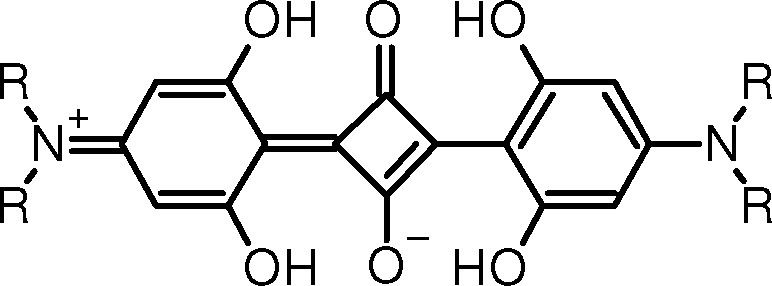
\includegraphics[width = \linewidth]{images/nAlinoSquaraine.jpeg}
\captionof{figure}{asdf\cite{doi:10.1021/acs.jpcc.2c03665}}
\label{SQstructureBasic}
\end{Figure}


\printbibliography
\end{multicols}


\end{document}




